\documentclass[letterpaper, 10 pt, conference]{ieeeconf}  % Comment this line out if you need a4paper

%\documentclass[a4paper, 10pt, conference]{ieeeconf}      % Use this line for a4 paper

\IEEEoverridecommandlockouts                              % This command is only needed if 
                                                          % you want to use the \thanks command

\overrideIEEEmargins                                      % Needed to meet printer requirements.

% The following packages can be found on http:\\www.ctan.org
\usepackage{graphics} % for pdf, bitmapped graphics files
%\usepackage{graphicx}
\usepackage[dvipdfmx]{graphicx}
\usepackage[dvipdfmx]{color}
\usepackage{epsfig} % for postscript graphics files
\usepackage{mathptmx} % assumes new font selection scheme installed
\usepackage{times} % assumes new font selection scheme installed
\usepackage{amsmath} % assumes amsmath package installed
\usepackage{amssymb}  % assumes amsmath package installed
\usepackage{multicol}
\usepackage{multirow}
\usepackage{url}
\usepackage{caption}
\usepackage[ruled,vlined]{algorithm2e}
%\include{pythonlisting}
\usepackage{algpseudocode}
\usepackage[dvipsnames]{xcolor}
\usepackage{cite}

\setlength\textfloatsep{5pt}

\title{\LARGE \bf
Time-Based Current Source (TBCS): A Highly-Digital PVT Adaptive Current Generator for Switched Capacitor Circuits
}

\author{Kentaro Yoshioka% <-this % stops a space
%\thanks{*This work was not supported by any organization}% <-this % stops a space
\thanks{
        {\tt\small yoshioka@elec.keio.ac.jp}}
}

\begin{document}

\maketitle
\thispagestyle{empty}
\pagestyle{empty}

%%%%%%%%%%%%%%%%%%%%%%%%%%%%%%%%%%%%%%%%%%%%%%%%%%%%%%%%%%%%%%%%%%%%%%%%%%%%%%%%
\begin{abstract}
VCO比較機ではdeadzone特性を使用することで自動的にIRN性能を入力に適した値に設定する。
The proposed adaptive time-domain (ATD) comparator automatically adjusts its input-referred noise performance according to the intermediate residual input level (?Vin) during conversion. Considering

入力に応じたオンデマンドのノイズと消費電力の比較器を提供。


\end{abstract}

%%%%%%%%%%%%%%%%%%%%%%%%%%%%%%%%%%%%%%%%%%%%%%%%%%%%%%%%%%%%%%%%%%%%%%%%%%%%%%%%
\section{Introduction}
スイッチドキャパシタ回路はパイプライン ADC、Pipeline-SAR ADCといった高精度・高速ADCの根幹を担う回路ブロックであり、5G、beyond 5Gといった先端通信回路を構成する\cite{ali201414, ali202012, lagos2018single, hung2020calibration}。基準電流源はこのようなスイッチドキャパシタ回路におけるオペアンプ特性を決定づける重要な回路である。特に高速なスイッチドキャパシタ回路であるとオペアンプの速度(ユニティゲイン)は重要な設計パラメータであり、注意深く設計する必要がある。しかしオペアンプ自体の設計に加え基準電流源のPVTばらつき性能は大きくスイッチドキャパシタ速度に寄与する一方であまり文献で注目されてはいなかった。

基準電流源は主にbeta-multiplierか電圧電流変換と2種類の設計アプローチがある。self-bias方式で電流を生成するbeta-multiplierは抵抗とトランジスタの温度特性が相補的であることを利用し、温度依存性をキャンセルする\cite{azcona2014precision, osipov2016temperature}。また電圧電流変換アプローチはPVTばらつきの影響が少ないBGR電圧源で生成した基準電圧を元に抵抗を用いて電圧ー電流変換を行う\cite{banba1999cmos, ueno2009300}。一方で両方の方式でも生成電流は抵抗値に応じて決定される。一般的な電流源は数10uAオーダであり、数10kオームのポリ抵抗阻止が用いられる。しかしこれらの抵抗値は量産時に製造ばらつきによって抵抗値は±50\%ほどばらついてしまい、そのドリフトは生成電流に直接現れる。

そのためこのような抵抗ばらつきは出荷テスト時にキャリブレーションするか設計マージンとして許容するのが一般的である。しかし前者は高コストなアナログテスト工数の増加を招き、後者はオペアンプのオーバーデザインにより消費電力、面積、歩留まりを悪化させる。電流源に用いる抵抗をトランジスタで置き換える研究も存在するが\cite{hirose2010nano, osaki20131, choi201423pw}、マッチングやアナログ特性が重要であるため回路面積は大きいためCMOSスケーリングに応じたコスト削減が難しい。

本論文ではhighly-digitalで低コストな電流源を実現するため、時間情報を基準とする電流源(TBCS)を提案する\cite{yoshioka201728}。具体的にはcurrent-starved inverterをADCのサンプルクロックでロックするDLL(delay-locked-loop)を構築し、セトリングした電流値を直接基準電流として用いる。current-starved inverterの遅延は電流と負荷容量で決定されるため、遅延を一定値にロックすることで一定電流を供給するレファレンスを構築できる。重要なことにTBCSはPVTに対し\textit{適応的}な電流生成を行うという特徴を持つ。負荷容量が増加するようなPVT条件の場合、本電流源は遅延を一定に保つため生成電流は増加する。これは増加したオペアンプに対しても増大した負荷容量の影響をキャンセルし速度一定に保つ効果がある。TBCSはほぼインバータセルとデジタル回路で構成でき、高いCMOS親和性を持ちプロセススケーラビリティは高い。試作回路は28nmCMOSにおいて面積はたったの$1200um^2$でありながらPVTばらつきに対し頑強であった。

Ref.\cite{yoshioka201728, yoshioka2019digital}に対し本論文はTBCSについてextensiveな課題探索、解析を追加する。具体的には以下のような貢献をする。
\begin{itemize}
\item TBCSの原理、回路インプリについて深い議論を行う
\item 詳細シミュレーションによりTBCSをオペアンプとスイッチドキャパシタ回路に組み込んだ際の特性を報告し、PVT追従性を明らかにする
\end{itemize}
本論文の構成について述べる。2章では従来研究とそれらの課題について述べる。3章ではTBCSの原理について説明し、4章ではTBCSの回路インプリについて議論し最後に5章でシミュレーション結果と解析について報告する。

%\section{Comparison of systematic comparator power consumption}
\section{Related researches}
\begin{figure}[!]
\centering
 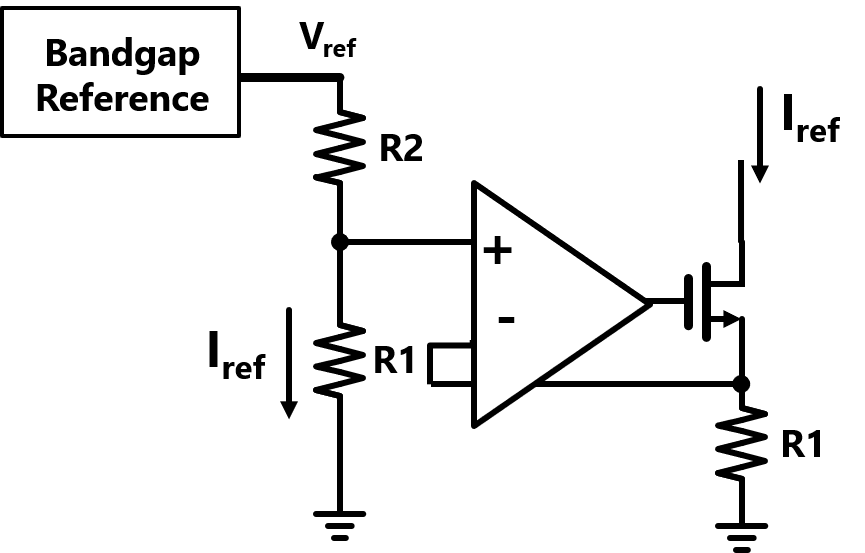
\includegraphics[width=0.5\textwidth]{figs/fig1.png}
  \caption{電圧-電流変換を用いたバンドギャップレファレンス型電流源}
\label{bandgap}
\end{figure}

\begin{figure*}[!]
\centering
 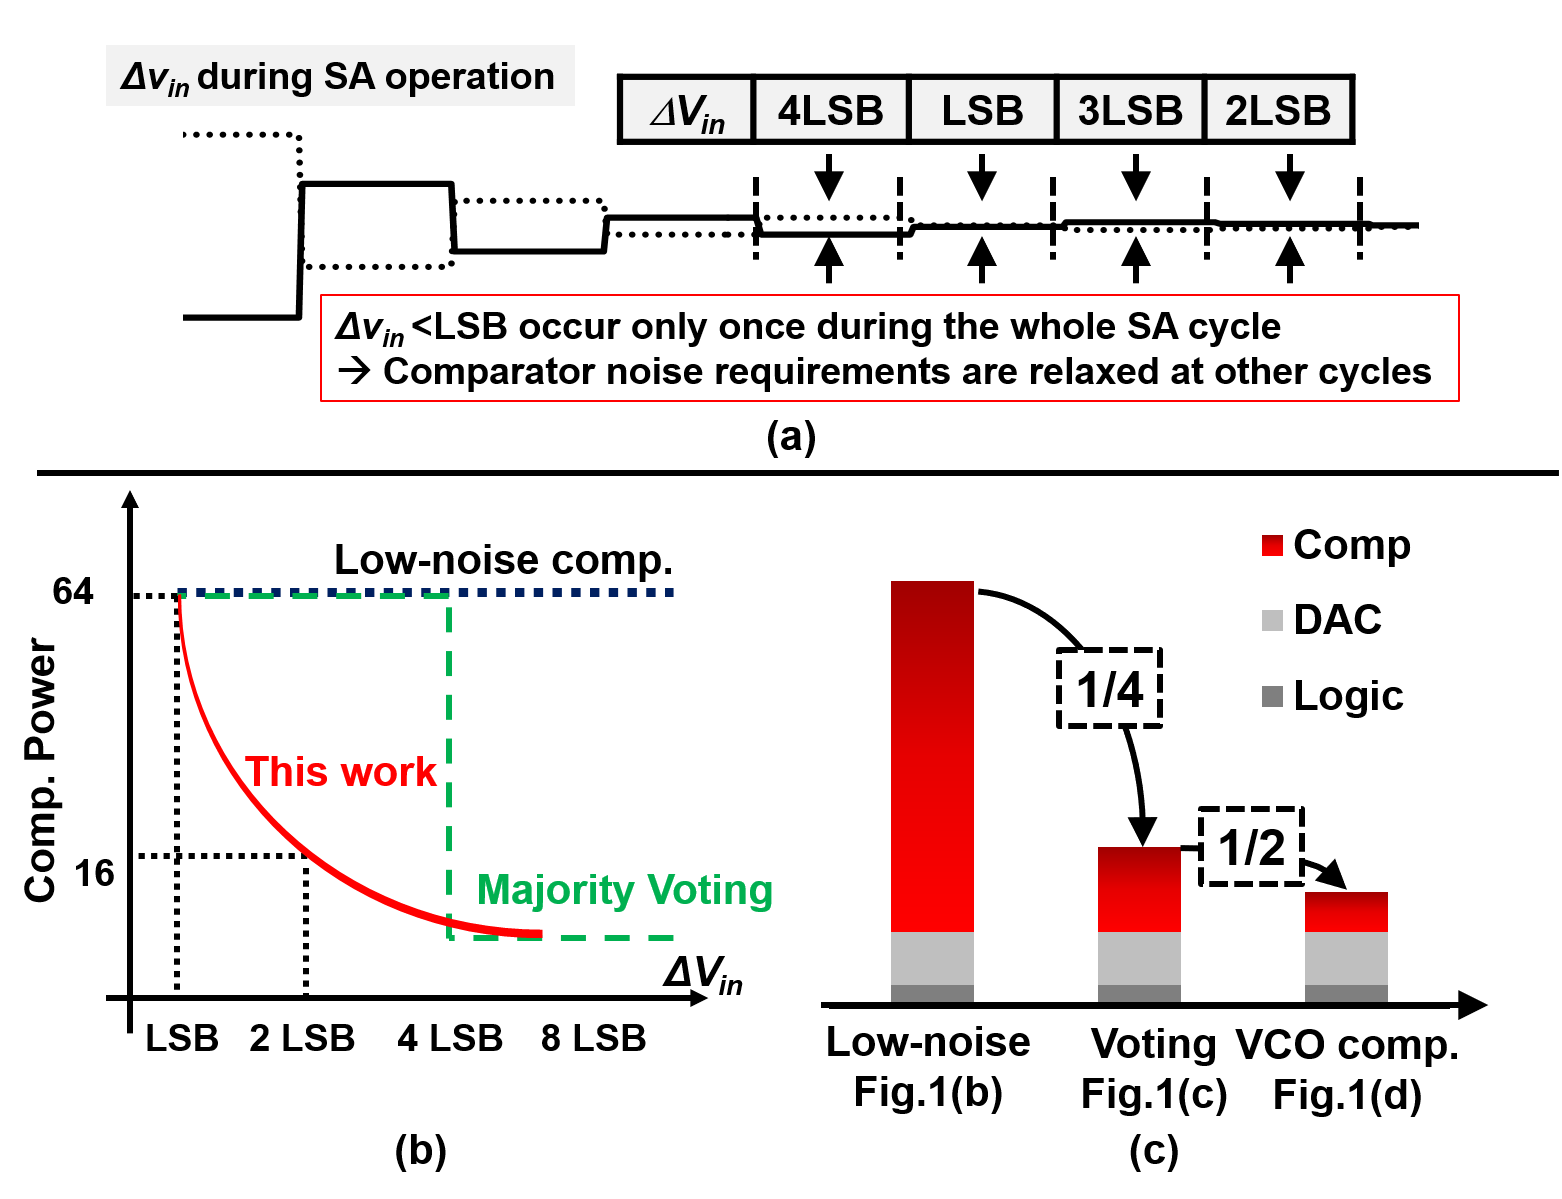
\includegraphics[width=0.9\textwidth]{figs/fig2.png}
  \caption{TBCSのブロック回路図。Current starved delay chainの遅延をCLKの半周期にロックするよう電流を制御する。遅延をロックした際の電流値は容量負荷に応じた値となりPVTばらつきに対して頑強であり、ロバストな電流源を実現できる。}
  \label{fig2}
\end{figure*}

\textbf{バンドギャップレファレンス} 広く電流源として使用されるバンドギャップ・リファレンスを図2に示す。バンドギャップ・リファレンス回路は参照電圧$V_{ref}$を生成し、
\begin{eqnarray}
    \centering
    I_{ref} = \frac{V_{ref}}{R_1 + R_2}
    \label{sar13b}
\end{eqnarray}
となる基準電流($I_{ref}$)を生成する。バンドギャップ・リファレンスは環境変動(温度、トランジスタしきい値、電源電圧等。以下PVTばらつきと呼ぶ)の影響を受けずに一定の電位を生成することができる。一方で抵抗値R1及びR2は製造ばらつきの影響を大きく受け、抵抗値はポリ抵抗であった場合最大で$\pm 40\%$程度ばらつく。そのため例えば$I_{ref}$=20uAをターゲットとした場合、max-min電流値はそれぞれ32uA、12uAと非常に大きな幅を持つ。このようなばらつきはオペアンプの設計マージンを拡大させ消費電力を増加する。

\textbf{適応的電流源技術} PVTに適応して動作する電流源技術はミックスドシグナル製品開発上重要であり、多くの研究がなされている。Ref.\cite{chuanyang,ron}はレプリカのアンプとチャージ用容量を用意し、オペアンプのスルーレートを直接観測することで所定のスルーレートを実現するよう電流にフィードバックをかけPVTに追従する適応的電流源を実現する。
一方でレプリカのオペアンプが必要となるため消費電力、面積のオーバーヘッドは大きい。一方でTBCSはレプリカアンプを用意することなく、ほぼデジタル素子を用いてPVTロバストな電流源を実現可能でオーバーヘッドは小さい。

\textbf{時間情報を用いたアナログ回路キャリブレーション技術} Ref.\cite{zhu}は基準クロックの時間情報を用いてアナログ回路素子をキャリブレーションする。具体的には電源電圧をDLLを用いて一定遅延になるよう制御し、基本的なアイデアはTBCSと同様である。
またDLLを用いて非同期SARクロックの遅延を制御し、DACセトリング時間をキャリブレーションする研究も存在する\cite{kapusta201314b,tompson}。
一方でオペアンプに用いる基準電流源のばらつきを時間情報を用いて抑え込む研究は著者の知る限りTBCSが初である。

\section{Time based current source (TBCS)}
\subsection{TBCS fundamentals}

図\ref{fig2}にTBCSの簡略化した回路ブロック図を示す。TBCSの必要な入力は所定周波数のクロック$CLK$(ADCのサンプルクロック等)のみであり、Delay-Locked-Loop回路(DLL)と構成要素や動作は近い\cite{sidiropoulos1997semidigital, lee19942, razavi2018delay}。基準電流源はレファレンス電流($I_{ref}$)を作り出し、オペアンプといったコア回路に与える。またTBCSではcurrent-starved-delayline(CSD)にも$I_{ref}$を与え、CSDは$CLK$に対し遅延を加えた$CLK_{CSD}$を出力する。この$CLK_{CSD}$に加わる遅延はCSDのステージ数を$N$としステージ遅延を$t_{DL}$とした場合、$Nt_{DL}$と表される。ここで$I_{ref}$が大きいほど$t_{DL}$は小さくなりその逆も然りである。そして$CLK_{CSD}$とCLKの反転出力($CLK_B$)間で位相比較を行い、遅延($Nt_{DL}$)がCLKの半周期時間$T_D$に漸近するよう基準電流源を制御し遅延を一定値に収束させる。

%TBCSは遅延器出力CLKDとCLKの反転出力(CLKB)間で位相比較を行い遅延(10*tDL)をCLKの半周期(TD)に漸近するよう電流を制御する。図 3右下にTBCSのプリンシパルとなる遅延器の電流-遅延特性を示す。

\begin{figure}[!]
\centering
 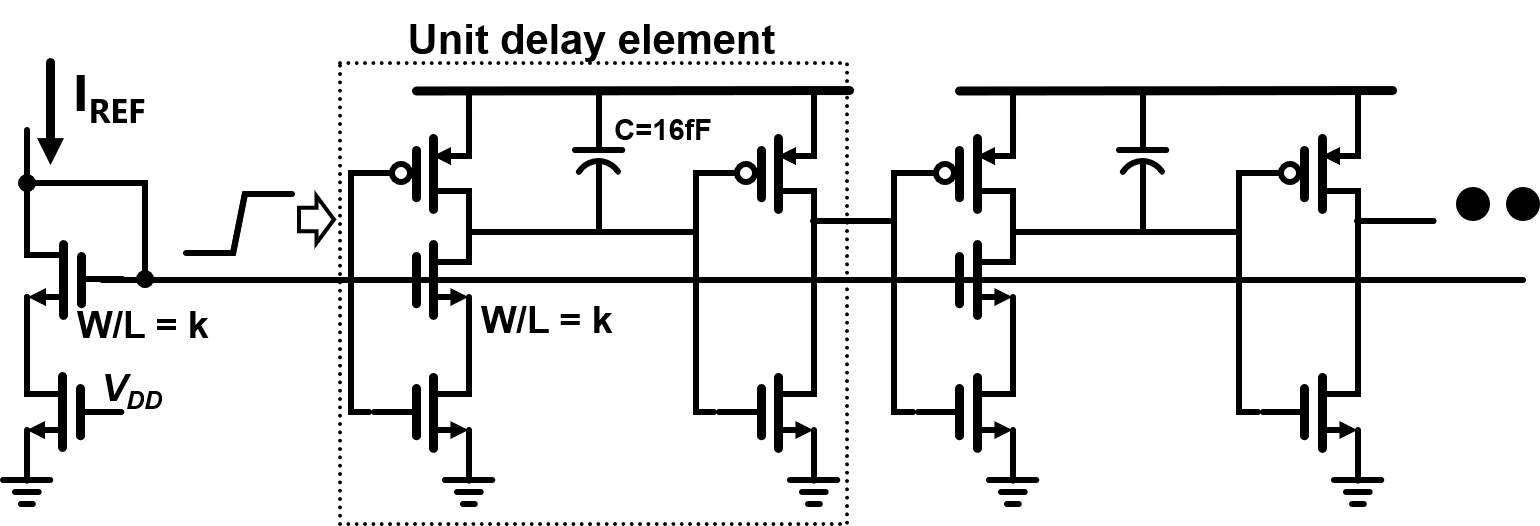
\includegraphics[width=0.5\textwidth]{figs/inv.png}
  \caption{(a) 
}
\label{inv}
\end{figure}

ここでCSDの遅延特性を考察することでTBCSが図\ref{fig2}右下に示すように環境に依らないロバストな電流生成が可能であることを示す。
図\ref{inv}にCSDの回路図を示す。容量負荷$C$を駆動するcurrent-sturvedインバータ(CSI)\cite{mroszczyk2014tunable}とインバータの接続で構成される。大信号特性を元にCSDの遅延$t_D$は次段インバータのオンしきい値を$V_{th}$とし、後段インバータ遅延を$t_{inv}$とすると
\begin{eqnarray}
    \centering
    t_D = \frac{V_{th}C}{I_{Ref}}+t_{inv}
    \label{delay}
\end{eqnarray}
と表せる。CSIの電流源が三極管領域に入る頃には信号は次段へと伝搬しているため、その影響は解析にて無視できる。ここで$t_{inv}$が前項より十分小さくインバータしきい値のばらつきも小さいと見なすと、$t_D$は$C$と$I_{ref}$によって決まると見なせる。そしてTBCSは$t_{DL}$を$I_{ref}$制御により一定値にロックするため、ロック時の$I_{ref}$は容量$C$に応じた値となる。先端CMOSプロセスにて容量は抵抗やトランジスタよりも電圧、温度、ミスマッチといった環境変動の影響は少ない。そのためTBCSは遅延ロック制御により環境変動によらない一定なロバストな電流生成を実現する。

上記eq.\ref{delay}よりTBCSのばらつき要因には 1)負荷容量のばらつきと2)次段インバータ遅延、オンしきい値ばらつきが存在する。
(2)の次段インバータの遅延はCSI遅延より1桁小さいため影響は少ない。一方で、TBCSがロバストな電流源となるためには容量絶対値ばらつきが小さいことが求められる。例えばmetal-insulator-metal(MIM)容量はミスマッチ自体は少ないものの、容量絶対値ばらつきが大きくTBCSにはそぐわない。一方で先端CMOSプロセスの配線間容量で作成するmetal-oxcide-metal(MOM)容量は絶対値ばらつきはMIM容量や抵抗素子よりも小さくTBCSに好適であり、ロバストな電流源を実現できる。また次節にて容量ばらつきによる電流変動がオペアンプ特性の一定化に役立ち、TBCSはPVTに適応的な性質を持つことを示す。

\subsection{PVTに適応した電流生成}
\begin{figure}[!]
\centering
 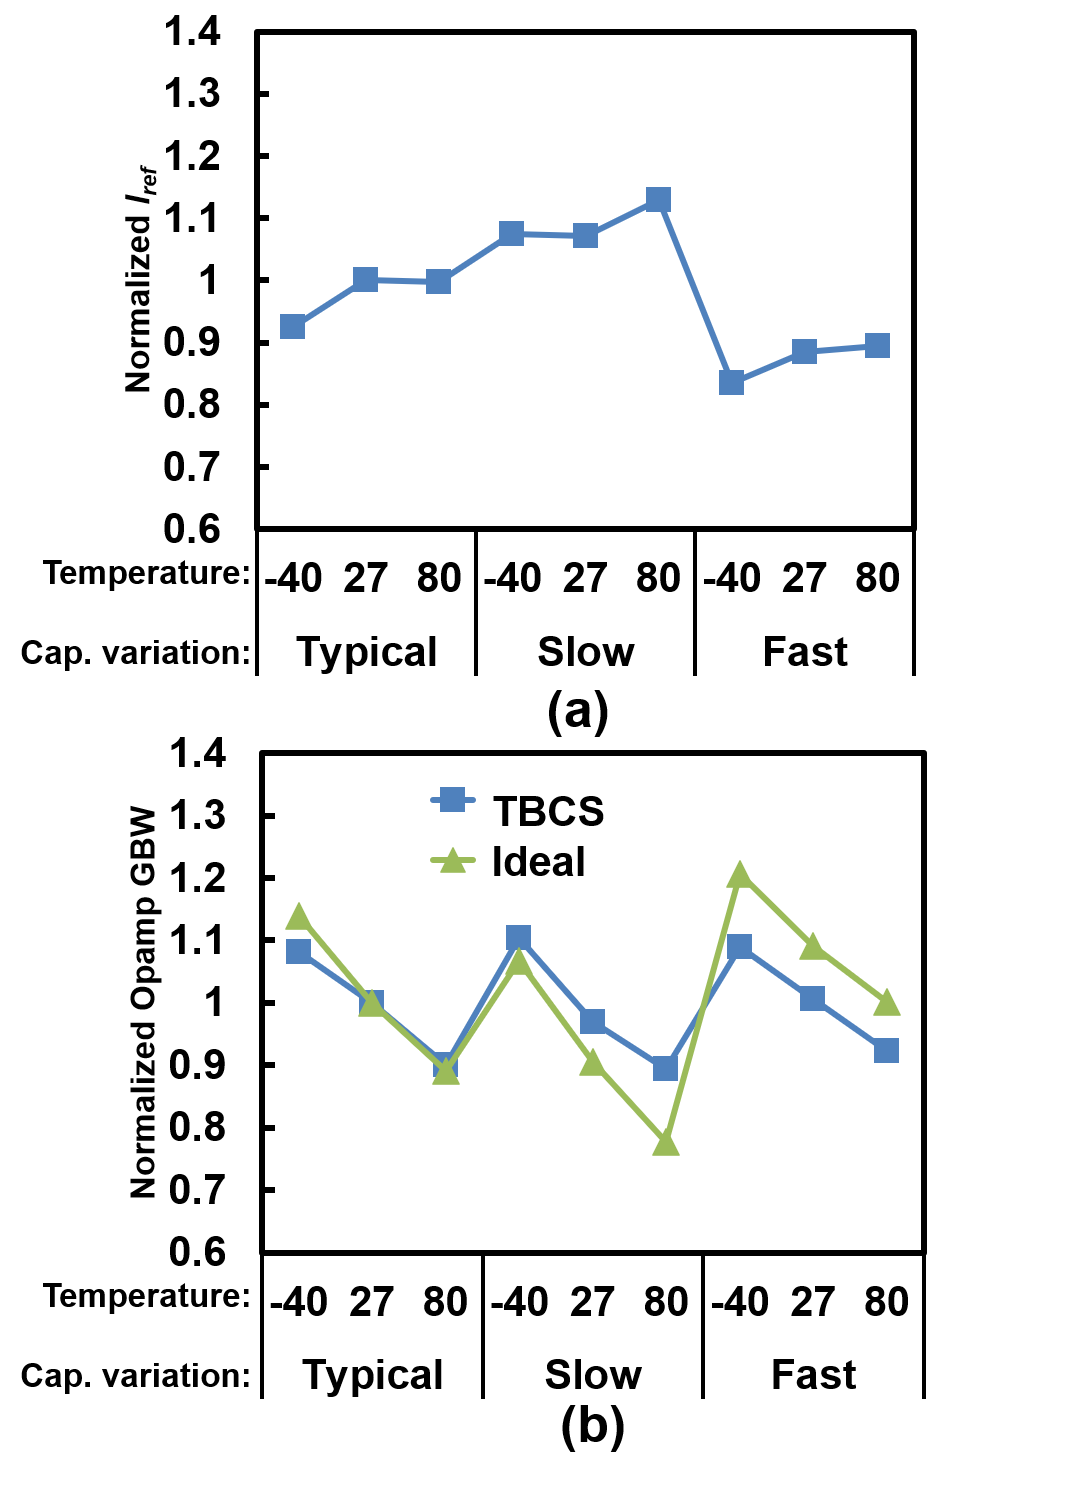
\includegraphics[width=0.5\textwidth]{figs/iref_var.png}
  \caption{(a) 
}
\label{cvar}
\end{figure}

TBCSはトランジスタや抵抗のPVTばらつきの影響は受けづらい反面、遅延が負荷容量の充電時間によって決まるため容量値ばらつきで生成電流が変動する。しかし興味深いことにTBCSの容量ばらつきの電流変動はオペアンプのPVTばらつき耐性を高めるよう作用し、このようなTBCSのPVT適応した電流生成について本節で解析する。
遅延の式eq.\ref{delay}より$C$が増えるとTBCSの生成電流も増加し反対に$C$が減ると電流も減る。このような特性は一定の電流を生成する基準電流源という視点では望ましくない。一方でこのような容量ばらつきが起きる時、スイッチドキャパシタ回路のオペアンプにおける負荷容量も同様に増減することに注目する。負荷容量が増加するとオペアンプのgain-bandwidth(GBW)は悪化してしまうが、TBCSはその減少分を補償するよう電流を増やすためPVTばらつきを通じGBWを一定に保つように働く。

この効果を更に解析するシミュレーションを実施した。図\ref{cvar}(a)に負荷容量が増大する条件のTBCS生成電流をプロットし、図\ref{cvar}(b)に同ばらつき下におけるオペアンプGBWの変動をシミュレーションした結果をそれぞれ示す。Slowは負荷容量大、Fastは負荷容量小のばらつき条件をシミュレーションである。SlowにてTBCSの生成電流は10-15\%ほど増加するが、この電流増加は負荷容量増大によって悪化したオペアンプのGBWを補償する。興味深いことにTBCSは一定電流を生成する理想電流源よりもオペアンプGBWをPVTを通し一定に保つ効果がある。反対にFast条件ではTBCSの生成電流は減少するもののオペアンプ負荷容量も減少するためGBWへの影響は小さい。Fast条件においては必要オペアンプGBWを維持しつつ消費電力を抑えるようTBCSは作用する。

一般的に大量生産チップではオペアンプのGBWといったクリティカルな性能指標をワースト条件でも仕様を満たすよう設計する。そのためワースト条件(Slow 80℃)におけるGBW悪化を抑えられるほど設計マージンを減らしチップ消費電力を改善できる。図\ref{cvar}(b)では理想電流源よりもTBCSを用いることでワースト条件のGBWを13\%改善することができ、設計マージン削減に大きく貢献する。

\subsection{CLK条件について}
また本設計では入力クロック周波数は80MHzを念頭においている。WiFi受信機をアプリケーションとして考えているため他に動作モードとしては20MHz,40MHzが考えられ、そのような周波数の時は電流源コードは最低値に張り付いてしまう。オペアンプは電流が最低値でも問題なく動作するように検証を行った。例えば80MHzを念頭に設計した遅延器で40MHzにてロックしようとすると2倍長い遅延を作成する必要がある。張り付きが生じてしまう理由は可変電流源のレンジ不足であり、そのような遅延を生成するために必要な電流に設定できないためである。可変電流源のビット数を増やしより小さい電流も生成できるようにすれば問題はない。

図 21 遅延器の意図的発振を行う場合の回路図

また周波数を問わず一定電流を生成したいケースもあり、対応方法を記述する。もし入力周波数が整数倍の関係性がある場合(無線受信機用ADC等)、遅延器を意図的に複数回発振させることで一定電流を生成可能である。入力クロックが設計周波数の1/4(ex:20MHz)であることが既知でその情報をカウンタに入力できるとする。図 21のようにクロックがHighになると遅延器はクロックのエッジ情報を伝搬し、最終段遅延器は初段遅延器に帰還をかけ発振する(奇数段発振器と同等)。この図では遅延器が発振し4回目のエッジで位相比較を行う。この動作により遅延器は80MHzと同じ遅延量でロックするためIREFも同等になる。4回目のエッジが検出されたあとはENABLEを立ち下げることで発振も中止される。例えば遅延器のN段目出力を用いて位相比較を行うことでfractional周波数においても電流生成が可能である。カウンタを制御するための周波数情報は前もって入力する必要はあるが一般的にPLLはそのような情報を元に周波数を生成しているため情報を得るのは容易い。

\section{Circuit Implementations}
\subsection{Control circuit and phase detector}
\begin{figure}[!]
\centering
 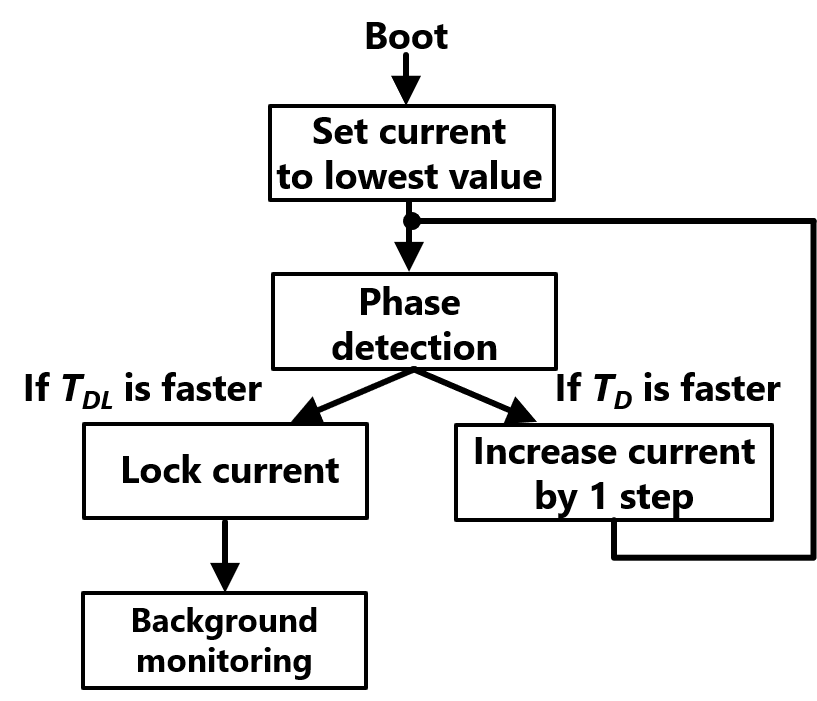
\includegraphics[width=0.5\textwidth]{figs/flowchart.png}
  \caption{(a) 
}
\label{flow}
\end{figure}
まずTBCSの基本的な制御について図\ref{flow}を用いて詳しく説明する。電源投入時には電流源の初期コードは最低値となり、そこから1コードずつ大きくしつつ最適電流コードを探索する。最初期は電流が小さいため$t_{DL}$は長く、$T_D$が早いと位相検知器は判定し電流を1コード分増加させる。この動作を$T_{DL}$が早くなると判定されるまで繰り返す。そして一旦を$T_{DL}$が早くなったと判定されるとバックグラウンド追従モードに入る。

この制御方法は単純なbang-bang制御であるが、収束までの時間が最大$2^N$サイクルかかる($N$は電流源のbit数)。今回実装する電流源は5bitのため、最大32サイクル収束に必要である。例えば逐次比較のようなアルゴリズムであれば収束にかかるサイクル数は短くすることができるが、動作中に温度等がドリフトしてしまうとリアルタイムで追従できないといったトレードオフがある。

\begin{figure}[!]
\centering
 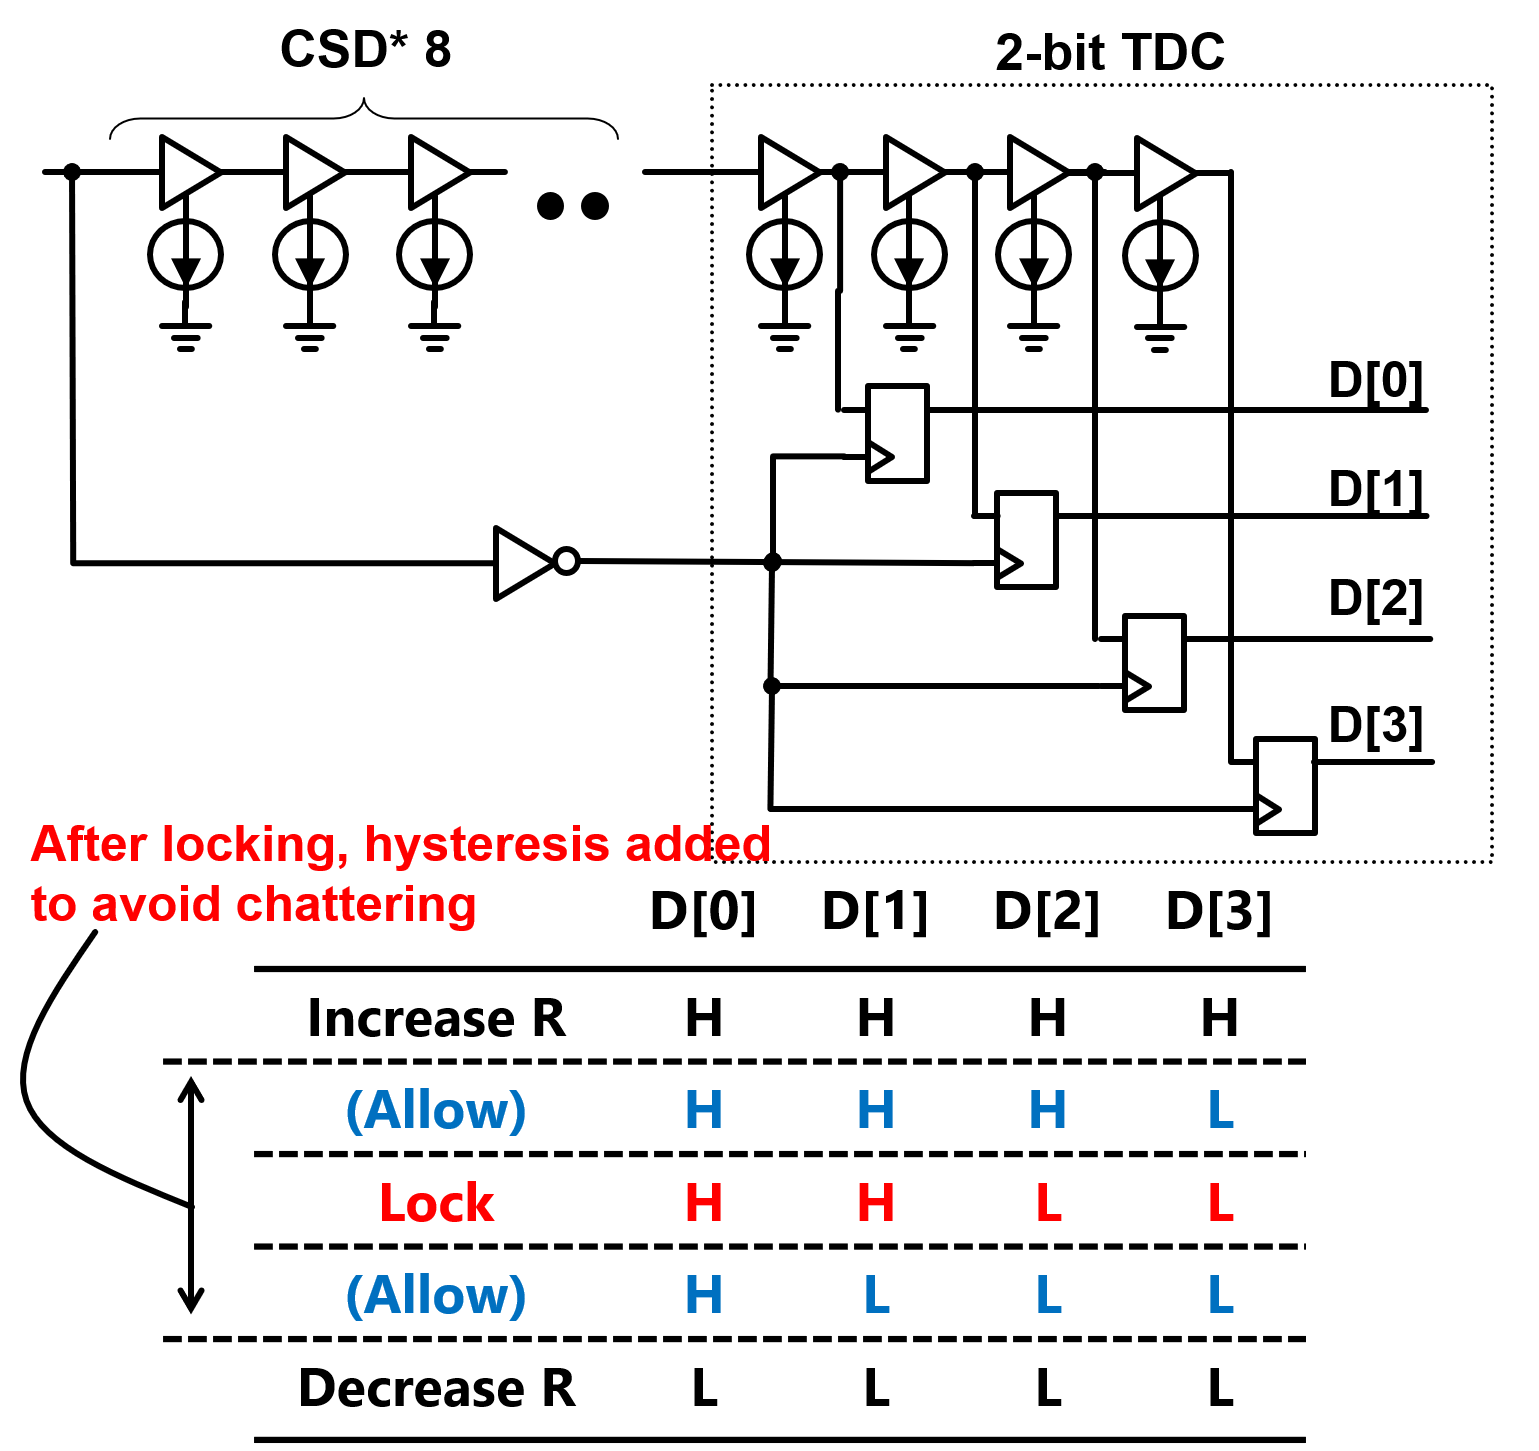
\includegraphics[width=0.5\textwidth]{figs/tdc.png}
  \caption{(a) 
}
\label{tdc}
\end{figure}

\begin{figure}[!]
\centering
 
\includegraphics[width=0.5\textwidth]{figs/chattering.png}
  \caption{(a) 
}
\label{chattering}
\end{figure}

次に位相比較器の実装について述べる。1-bitのTDCは簡単にフリップフロップひとつで実現できるが、コードばたつき(チャタリング)の可能性がある。図 \ref{chattering}にチャタリングの例を示す。これは誇張して遅延変化を書いているが、最初の位相比較で遅延量を減らすように制御をした場合(コード14→15へ)、次の位相比較時には遅延がTDに対し小さくなってしまう可能性がある。この場合位相比較結果を受けて再び電流コードを減らす(15→14へ)ように制御され毎サイクル電流値が変わり、スイッチドキャパシタ回路において不要なスプリアスが発生してしまう。例えば一度位相関係が逆転したら制御コードをロックすることでチャタリングは防げるが、それではPVTドリフトに対して追従することはできない。また一般的なDLLではループフィルタ\cite{sidiropoulos1997semidigital}やデジタルフィルタ\cite{kim20172}を用いて精微な遅延を生成するが、本回路ではPVTに適応する電流源の設計が主目的であり遅延の精度は重要ではないためこのようなフィルタは使わない。

本回路では図\ref{tdc}に示すように位相比較器をを2bit TDCとすることで電流源がロックした後のチャタリングを防止しつつPVTドリフト追従機能をもたせる。
本実装では$T_{DL}$が早くなり遅延がロックするとその後は長期的なPVT変動に対応するバックグラウンドモニタリングモードに移行する。ロック前はbit D[1]のみモニタし電流値を制御し、ロック後はTDCの2-bit出力D[0:3]を用いて環境変動に追従する。表にある通りD[0:3]が全てHighかLowになる時以外電流DACコードを更新しないことで細かなチャタリングを防ぎつつ、長期的な環境変動に対応する。

\subsection{R-DAC}
\begin{figure}[!]
\centering
 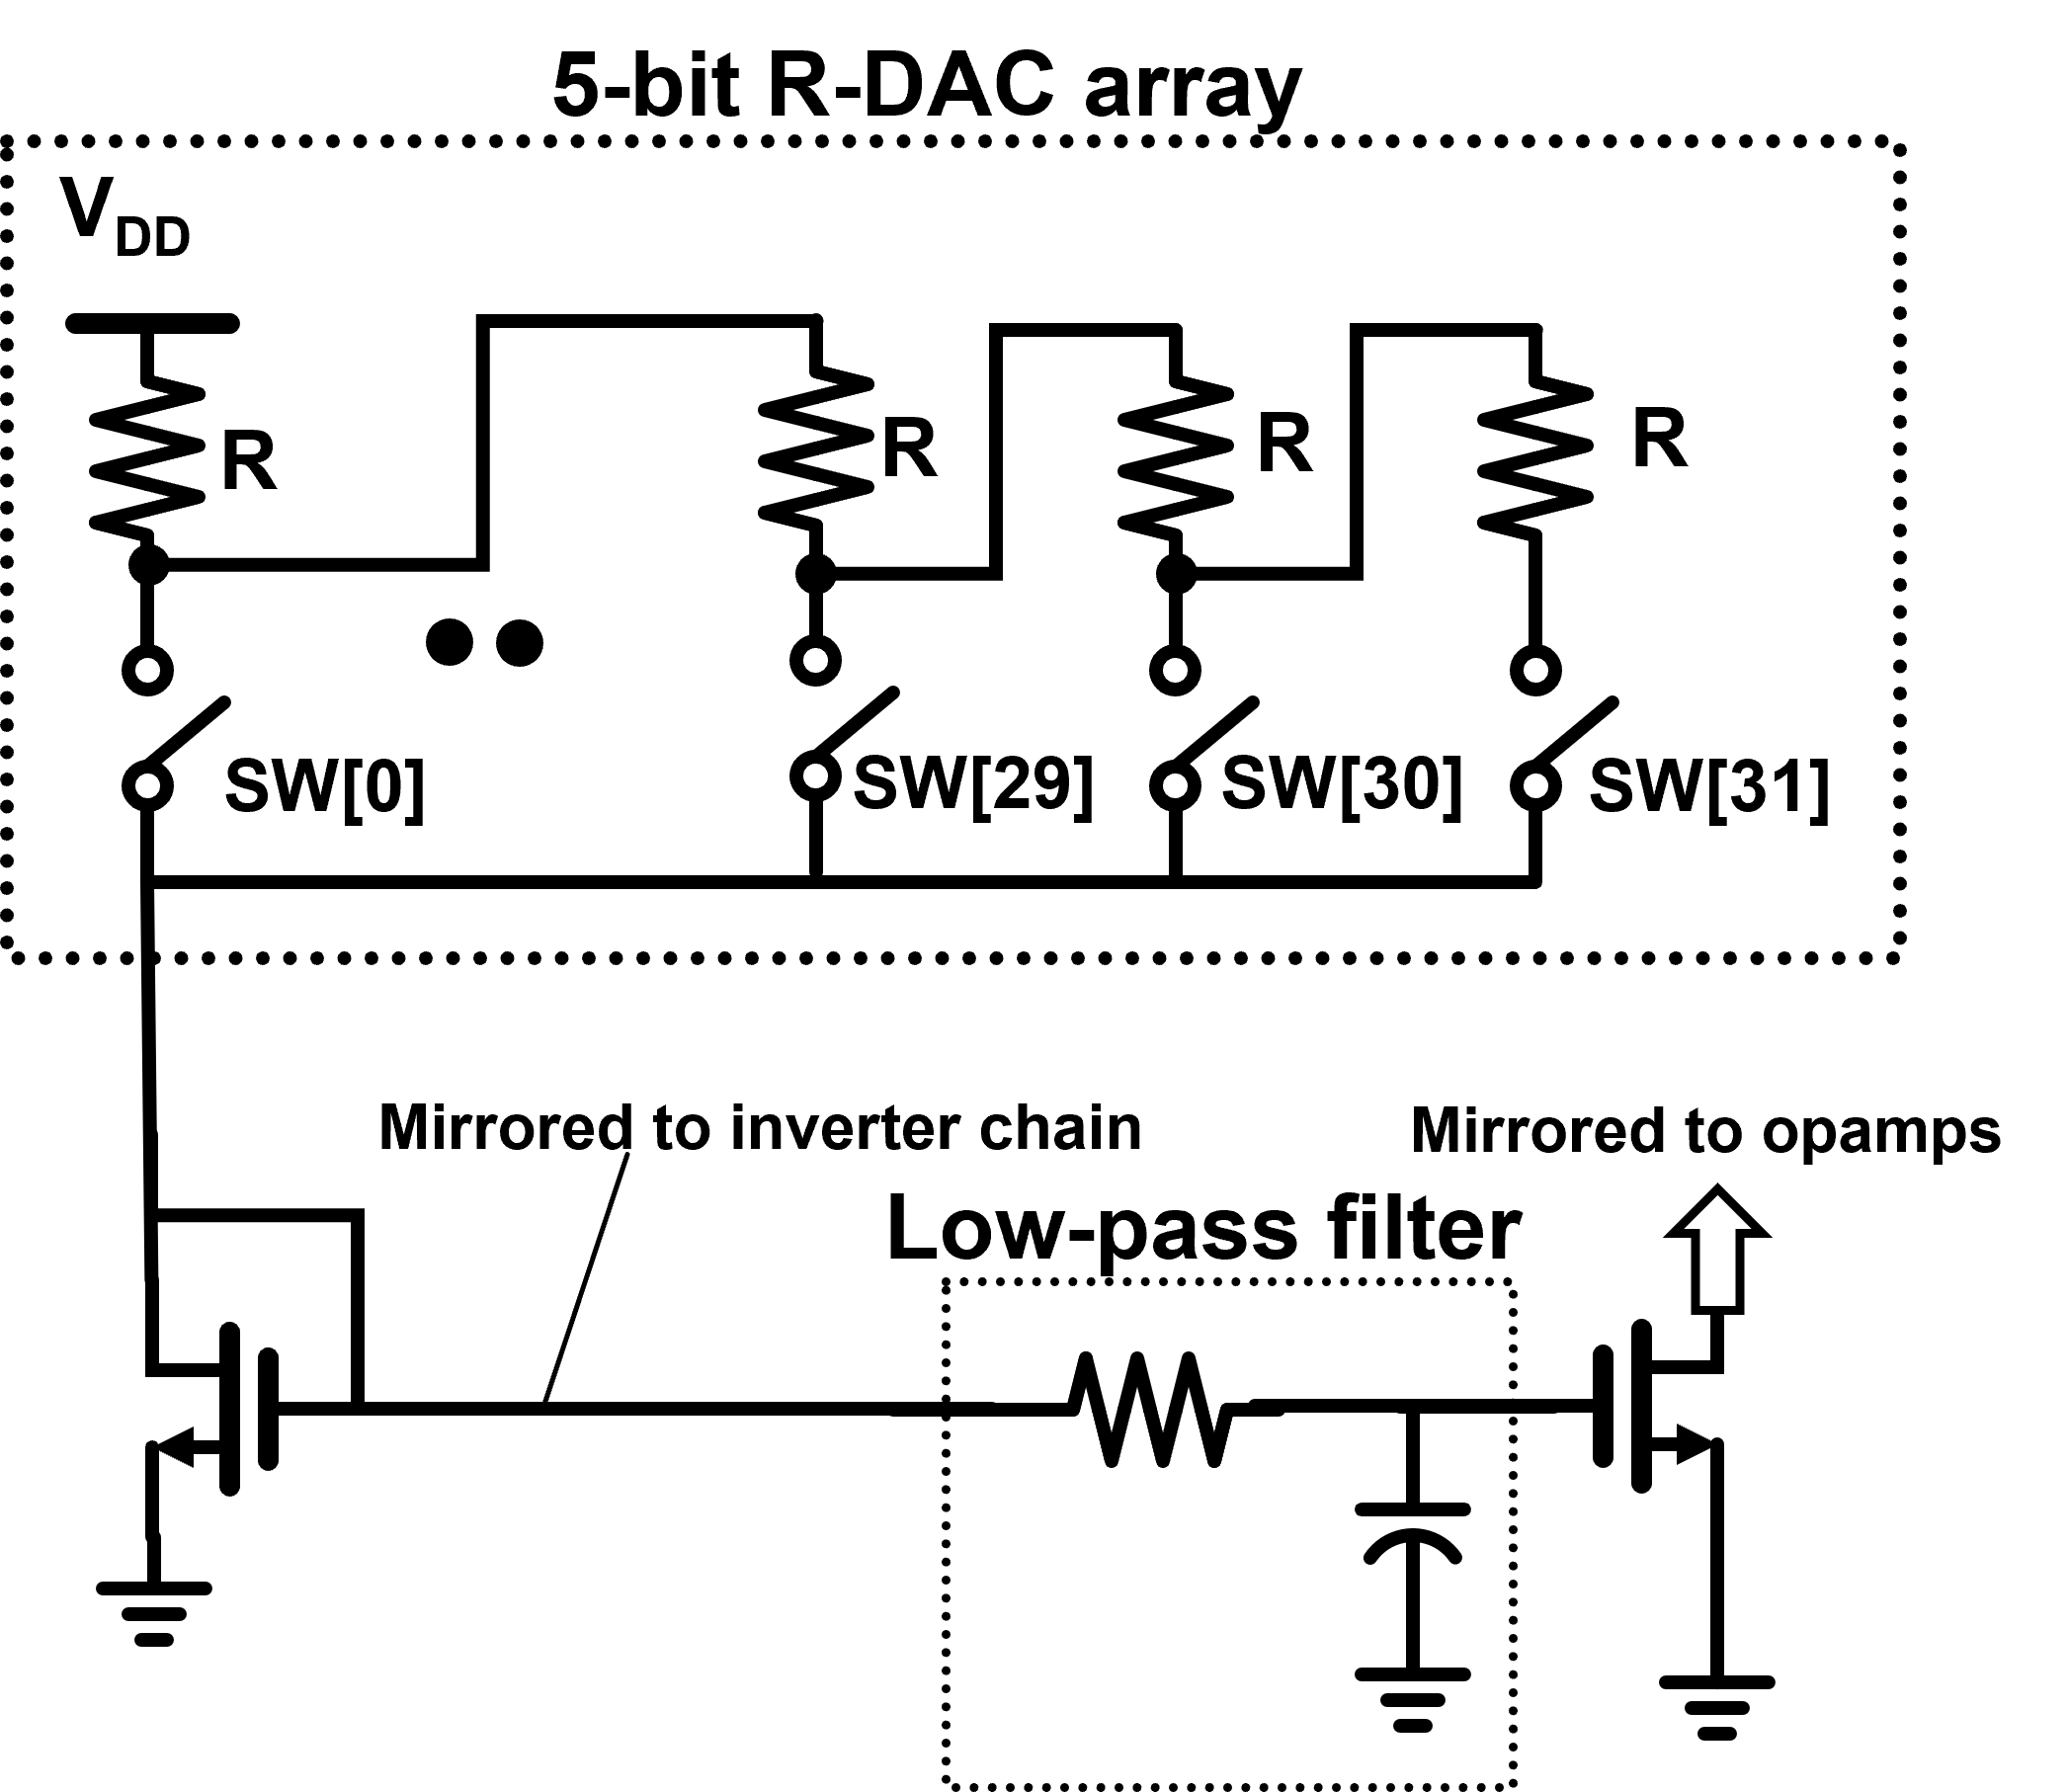
\includegraphics[width=0.5\textwidth]{figs/rdac.png}
  \caption{(a) 
}
\label{rdac_sche}
\end{figure}
可変基準電流源を構成するR-DACの回路図を図\ref{rdac_sche}示す。電流値$I_{ref}$は
\begin{eqnarray}
    \centering
     I_{ref} = \frac{V_{DD}}{R_{NMOS}+\sum R_{DAC}}
    \label{iref_eq}
\end{eqnarray}
で決定されR-DACの抵抗値を制御することで電流制御を実現する。R-DACはone-hotのデジタル制御コード(SW[0:31])によって制御され、SW[31]がHighの時RDACは32Rとなり最大値を示し、SW[0]がHighの時抵抗値は最低でRDACはRを取る。TBCSでは抵抗DAC設計が最もクリティカルな要素となる。具体的には(1)生成電流の精度が必要十分か、そして(2)抵抗ばらつき下でも目標電流値を生成できるかの2点を満たすようにR-DACは設計しなければいけない。

\begin{table}[]
\centering
 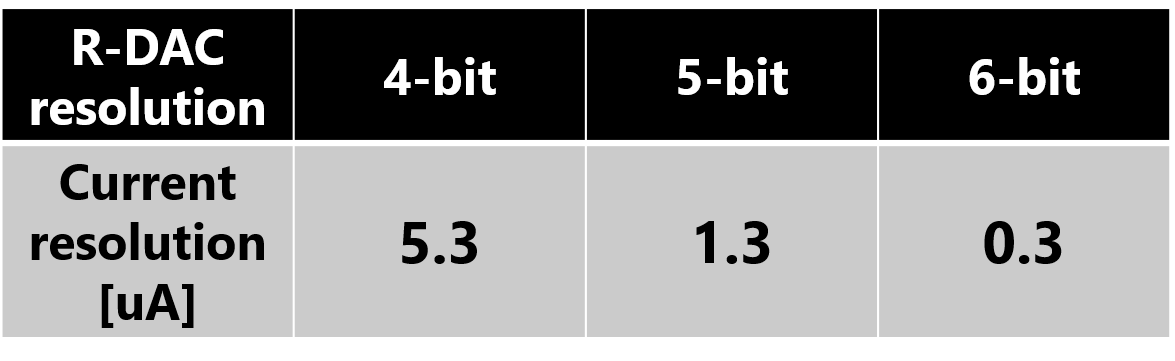
\includegraphics[width=0.5\textwidth]{figs/rdac_table.png}
  \caption{(a) 
}
\label{rdac_table}
\end{table}

まず(1)で述べたとおり式\ref{iref_eq}の通り抵抗DACの分解能は生成電流の分解能に直結する。R-DACを単位抵抗R=4kΩと一定で分解能を4,5,6 bitと変動させた際の電流分解能を表\ref{rdac_table}に示す。表では簡単のため中央コードにおける電流変分を採用した。今回の設計値では4-bit DACでは5uAとステップが大きすぎ設計にそぐわないものの、5-bitでは1.3uAと必要十分の精度が得られる。

\begin{figure}[!]
\centering
 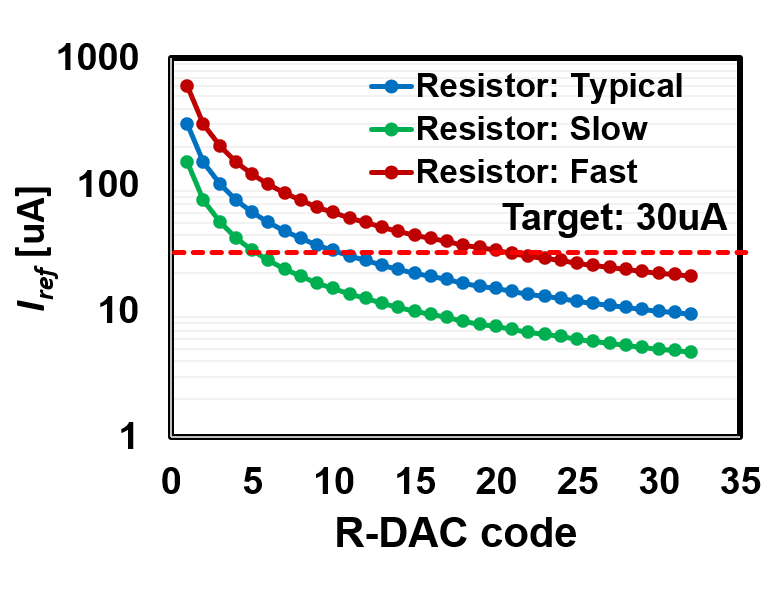
\includegraphics[width=0.5\textwidth]{figs/rdaccode.png}
  \caption{(a) 
}
\label{rdac_pvt}
\end{figure}

(2)に関しては抵抗のPVTばらつき下でも目標電流値にロックできるか確認しておく必要がある。図\ref{rdac_pvt}に抵抗のPVT におけるDACコードvs 生成電流をプロットした。今回目標とする30uAの電流生成はSlowからFast条件全てでカバーできることがわかる。もし抵抗ばらつきが大きくターゲットをカバーできないのならばR-DAC分化能を増やし抵抗可変範囲を広く取る必要がある。

また図\ref{rdac_sche}に示すとおりTBCSは抵抗をスイッチングするため、抵抗切替時に不要なスプリアスがオペアンプに伝搬してしまう可能性がある。そのような不要成分を取り除くため受動素子によりローパスフィルタを構成し、オペアンプへミラーするバイアスのスイッチング成分を除去している。

\subsection{Inverter}
最後に遅延素子について記述する。スケマを図\ref{inv}に示す。

・ミスマッチは重要な要素。電流生成ばらつきに直結する一方で今回のように1uA分解能の電流生成TBCSでは影響が少ない。

・Nステージの遅延器の場合、単体遅延器のミスマッチより生じる遅延ばらつきをvarとするとvar*sqrt(N)と増加。

一方で信号成分(合計遅延)はN倍になるため1/sqrt(N)とばらつきは緩和される。

今回の設計ではσ=30ps程度であり、TDCの単位ステップが600psに対し十分小さくTBCSの電流値への影響は少ない。

・同様にジッタもDLL等では重要な要素だがTBCSでは重要ではない。ジッタは遅延量に比べ十分小さく、それでいてTBCSがロック後にはヒステリシスがあるため遅延器とTDCのジッタは生成電流に影響は与えない。

%%%%
従来電流源では抵抗のミスマッチのみIREFに作用しており、そのようなミスマッチは小さく無視できた。しかし遅延器のトランジスタばらつきは無視できないほど大きく電流-遅延特性を変化させてしまう。モンテカルロシミュレーションでこのばらつきを見積もり、±3σのばらつきが生じた場合の電流値も同様にプロットした。FF、SFの高温条件において最悪値である12uA(typ値に対して25\%減)を記録するが、前述したとおりトランジスタが高速で動く条件のため電流が減少しても問題ない。同様に最高値もSS,SFの低温条件のみ発現するがオペアンプ速度を補填するため問題はない。

\section{Experiment and simulation analysis}
\begin{figure}[!]
\centering
 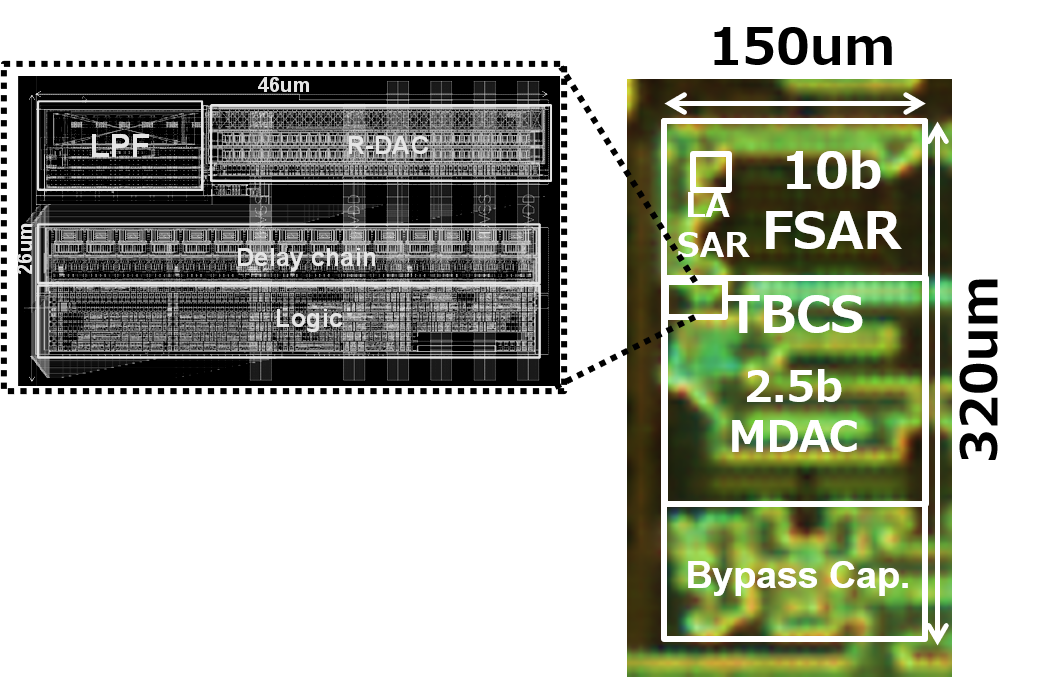
\includegraphics[width=0.5\textwidth]{figs/chip.png}
  \caption{(a) 
}
\label{chip}
\end{figure}

\begin{figure}[!]
\centering
 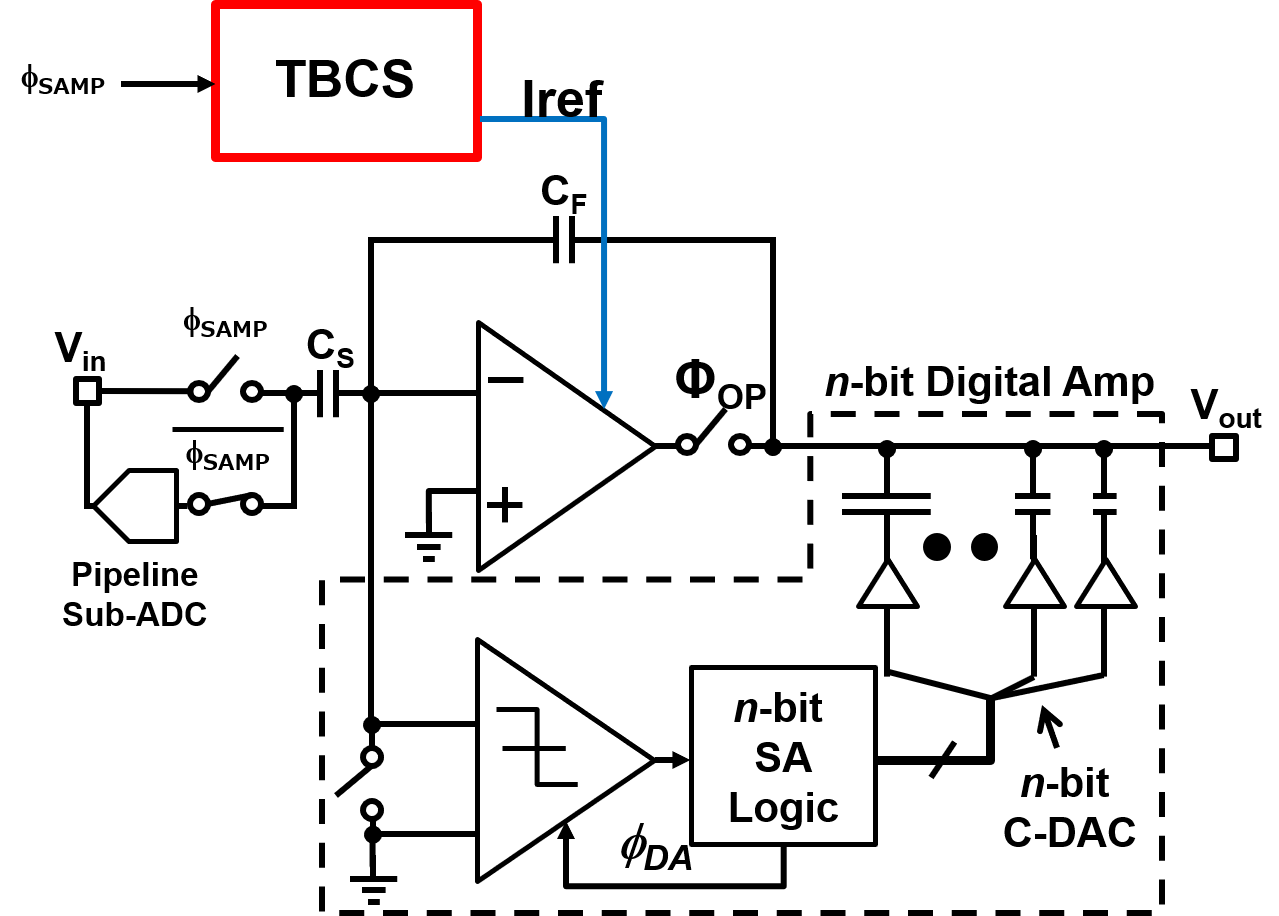
\includegraphics[width=0.5\textwidth]{figs/switchcap.png}
  \caption{(a) 
}
\label{scap}
\end{figure}

\begin{figure}[!]
\centering
 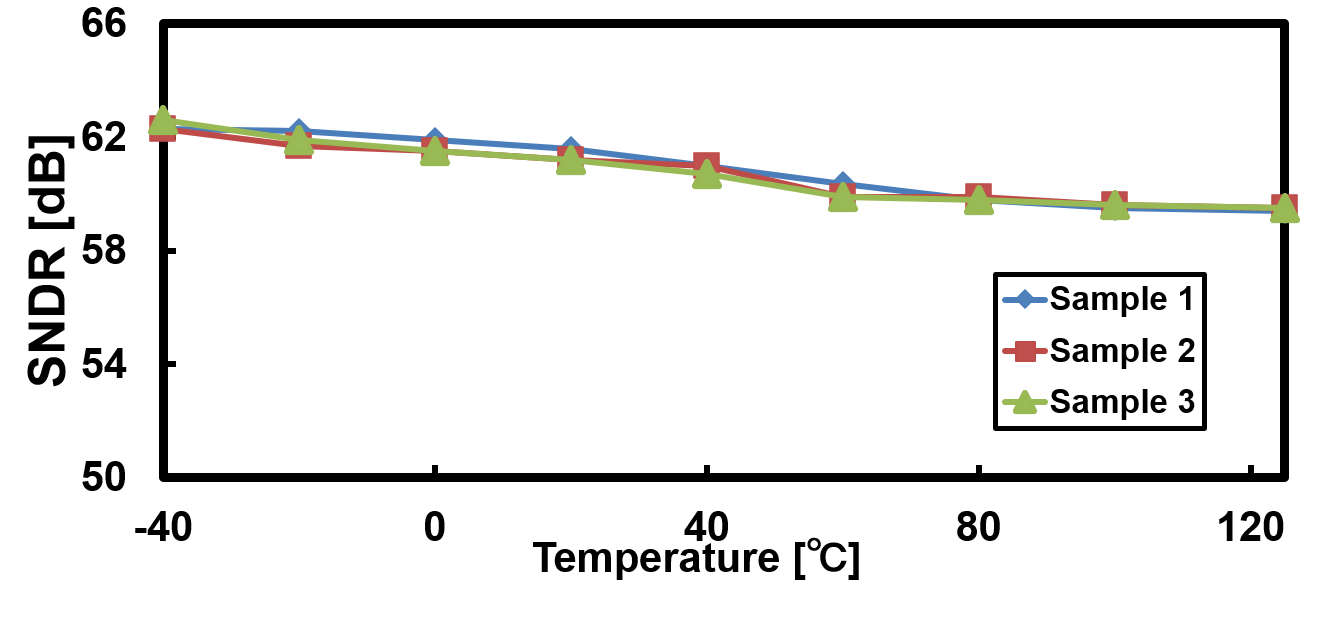
\includegraphics[width=0.5\textwidth]{figs/sndr.png}
  \caption{(a) 
}
\label{sndr}
\end{figure}

\begin{figure}[!]
\centering
 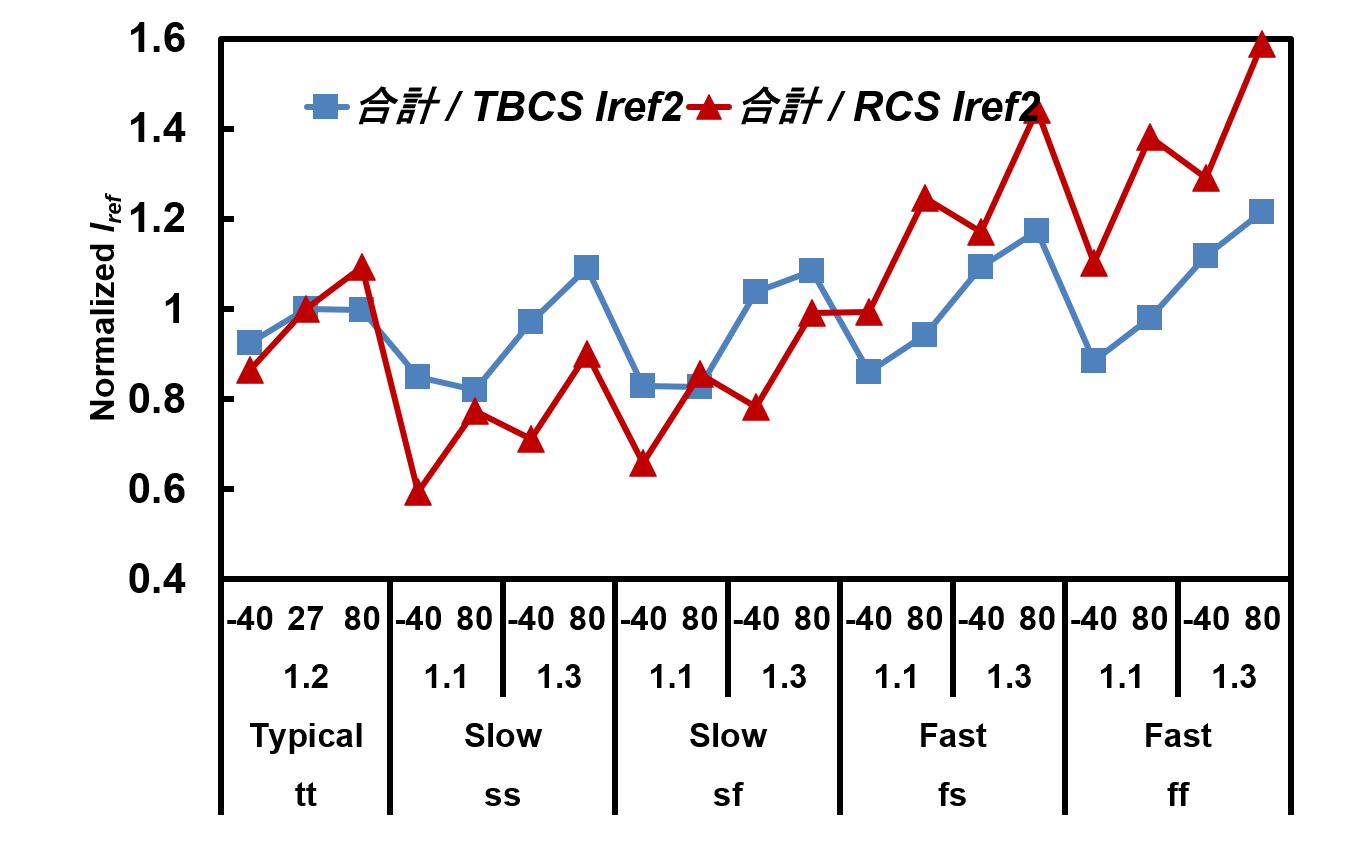
\includegraphics[width=0.5\textwidth]{figs/pvt.png}
  \caption{(a) 
}
\label{iref_pvt_both}
\end{figure}

\begin{figure}[!]
\centering
 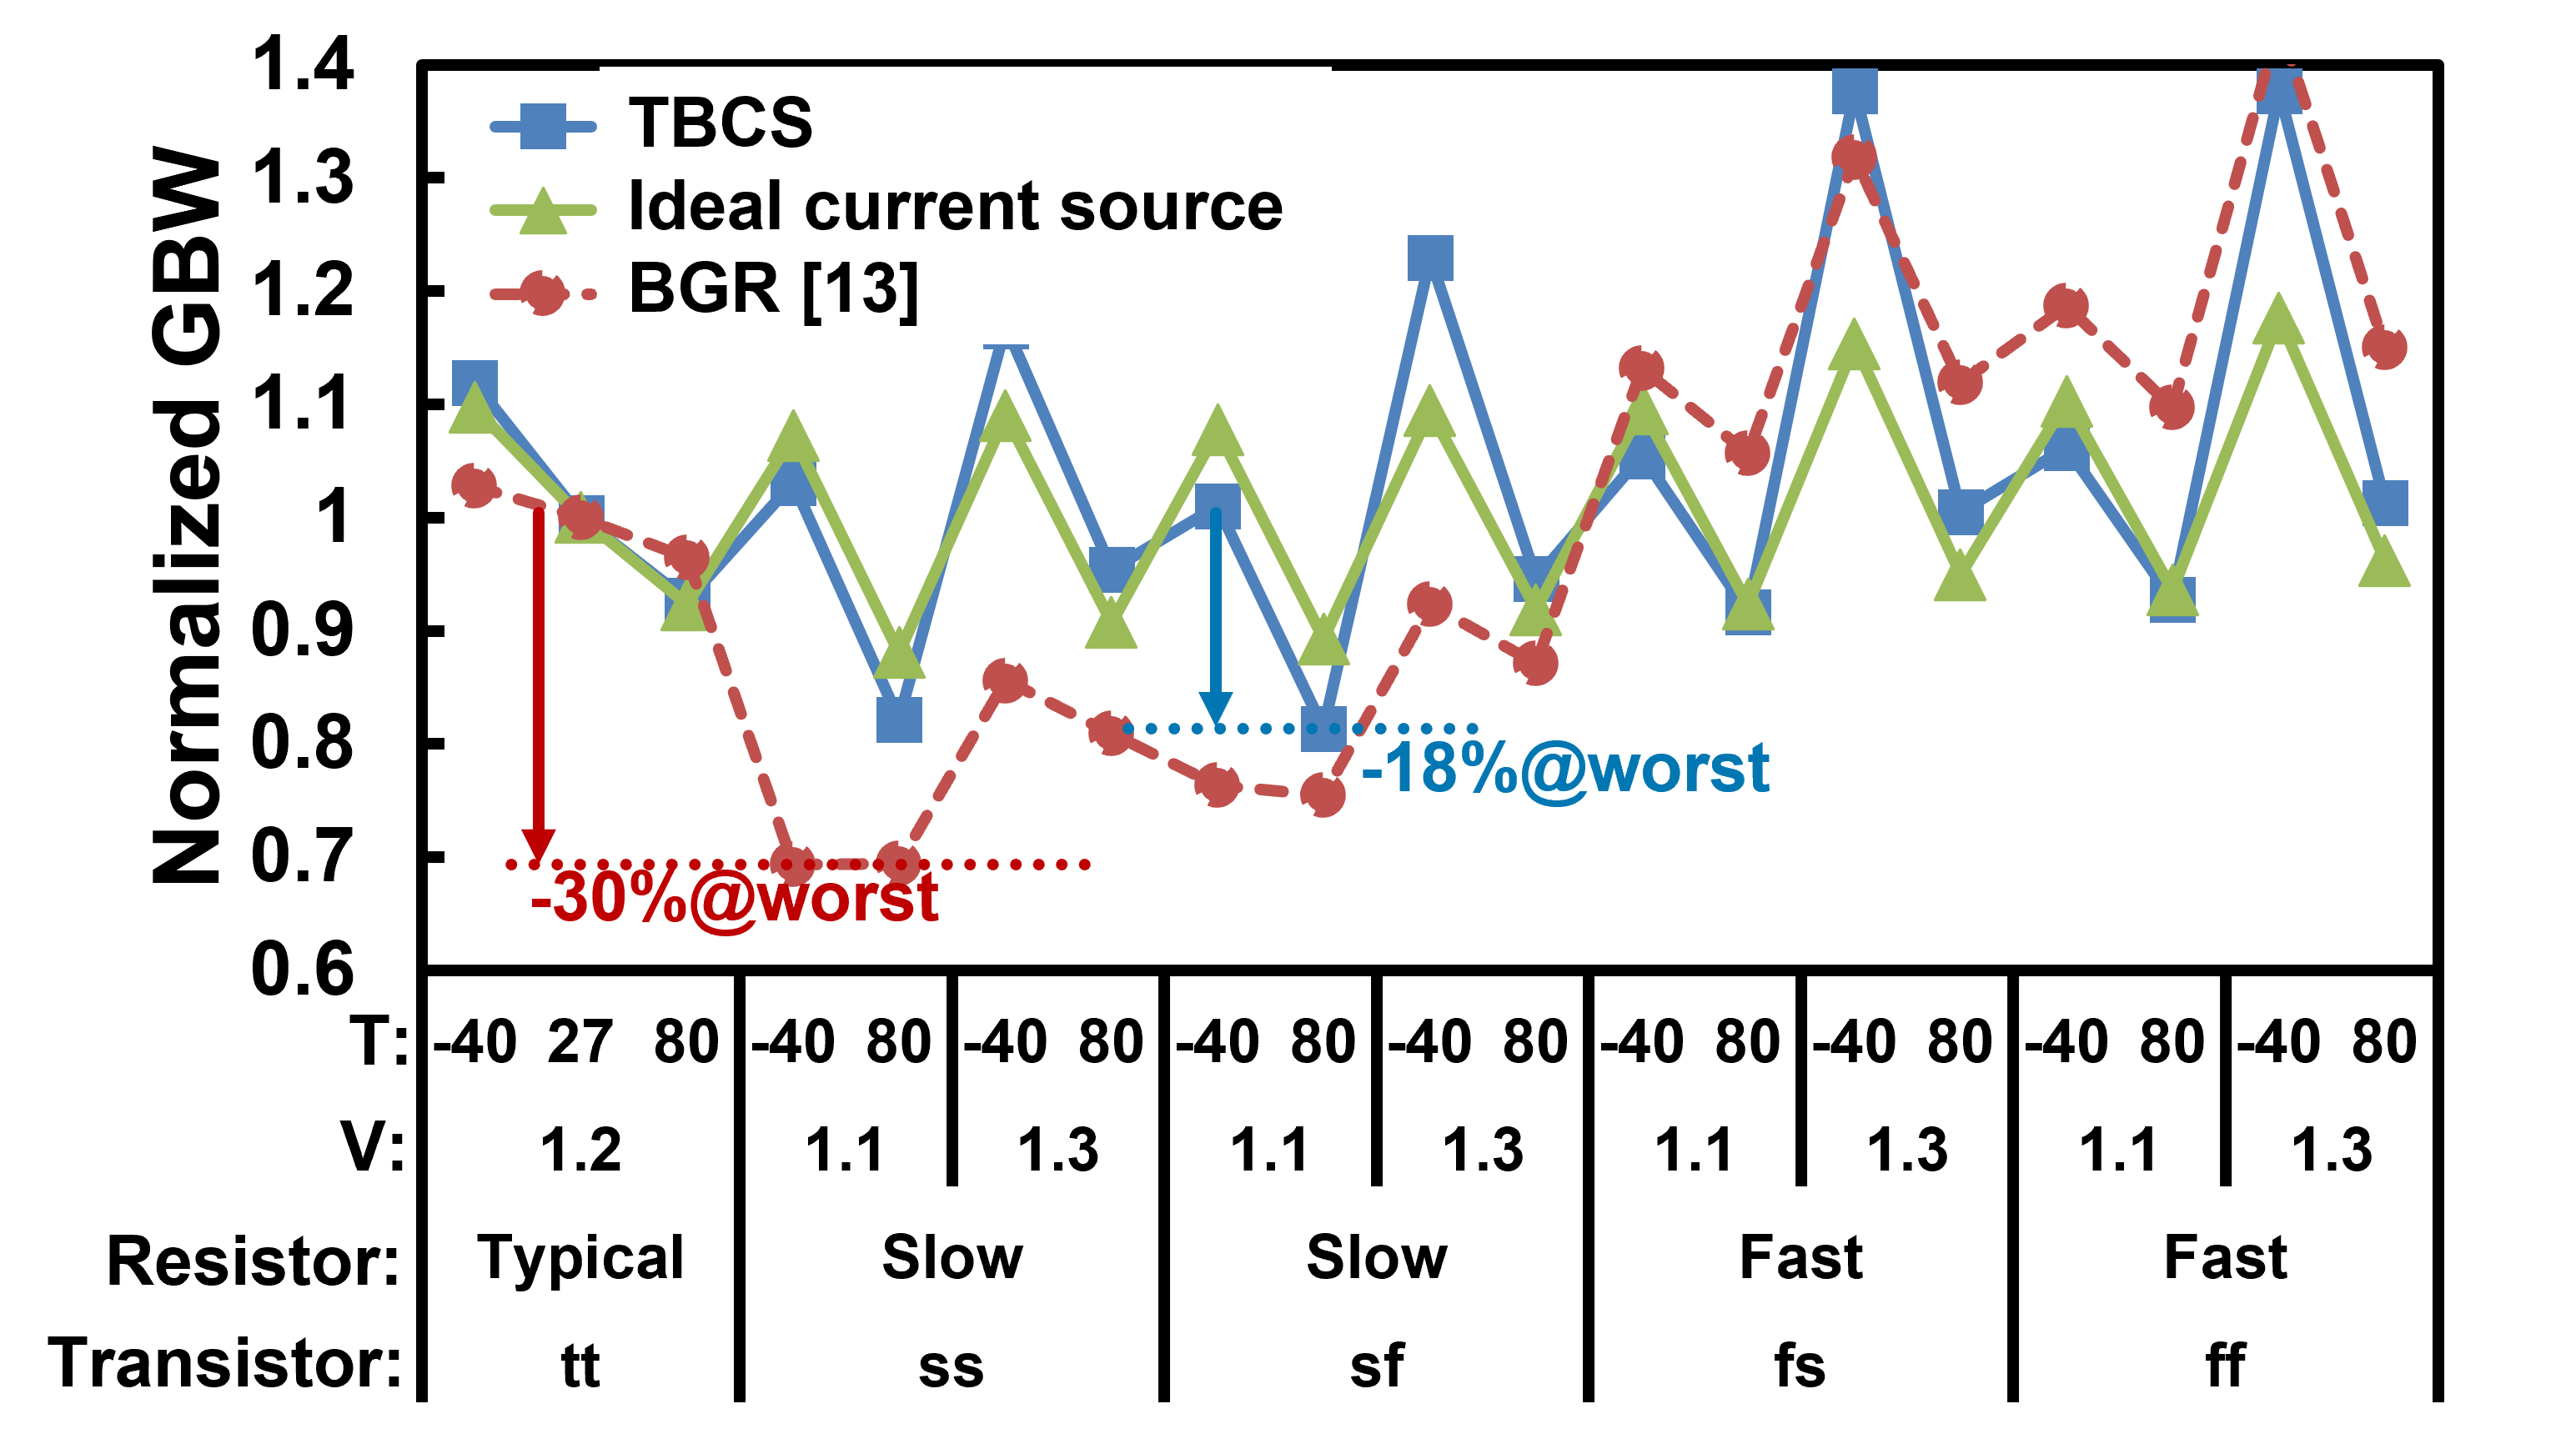
\includegraphics[width=0.5\textwidth]{figs/pvt_gbw.png}
  \caption{(a) 
}
\label{iref_gbw}
\end{figure}


% 試作と方針説明
提案回路を28nm CMOSを用いて試作しチップ写真とレイアウトを図\ref{chip}に示す。占有面積は46um x 26um(0.0012mm2)であり、非常に小さい。ロジックはRTL設計、ゲートネット生成、$P&R$とデジタル回路と同様のフローで作成した。TBCSはバンドギャップ・リファレンスと違いバイポーラトランジスタやオペアンプを必要としないため、先端CMOSかつ低電源電圧でも容易に設計できるのが特徴である。バイポーラトランジスタ、オペアンプはCMOSプロセスが微細化しても面積はスケーリングしないため相対的に高コストになってしまうが、TBCSはデジタル素子の占める割合が高く、微細プロセスほど低コストになる。

試作チップはref.\cite{yoshioka201728}に統合した形で行い、電流モニタリング端子は持たないためTBCSの詳細特性を測定することはできないため主な性能解析はシミュレーション結果を報告する。一方で幅広い環境変動におけるスイッチドキャパシタ動作とADC動作は実測で確認できており、そこからTBCSが問題なくファンクションしていることが伺える。ref.\cite{yoshioka201728}におけるPipelined-SARにおけるスイッチドキャパシタ回路とADCのSNDR評価結果を図\ref{scap}に示す。このスイッチドキャパシタ回路は二段階増幅を採用しており、荒い一次増幅をTBCSによりバイアスされたオペアンプが実施し精微な二次増幅を逐次比較回路が担っている。本回路ではオペアンプが動作していないと十分な精度は得られないが、測定結果図\ref{sndr}より-40~125℃のレン時でADCは高いSNDR(60dB)を達成しており正常にTBCS動作とスイッチドキャパシタ回路が行われていることがわかる。

% 電流源としての性能評価
まず比較のためFig.\ref{bandgap}のバンドギャップレファレンス型電流源(BGR ref)\cite{banba1999cmos}とTBCSのPVTばらつきに対する生成電流のシミュレーション結果を図\ref{iref_pvt_both}に示す。ポリ抵抗を用いたBGR refは温度や製造ばらつきに対する感度が大きく、max min電流値は15uA離れている。特にSSLTLV条件において電流値がtypに対し40\%低下してしまうのは非常に影響が大きい。
オペアンプ負荷のスイッチ抵抗増大等の効果もあり、オペアンプセトリング条件が最も厳しくなる条件で更に電流源値が20\%も低下してしまうとセトリングを満足するのは厳しい。オペアンプ設計時にはSSLTLV条件のセトリングを満足するようにスルーレートを設定するため、typ含む他条件においてスルーレートは過剰気味になってしまい電力オーバーヘッドが生じてしまう。

またFF条件において電流値が大きく増加してしまうのもオペアンプ設計にもおいて問題が生じる可能性がある。FFではトランジスタしきい値降下はあるものの、$I{ref}$が増大してしまうとその分各トランジスタの$V_{gs}$バイアス電圧を増加する必要がある。これはFF条件においてオペアンプの出力電圧範囲を狭めてしまう危険性をはらむ。オペアンプ電力を最小化するという観点ではSS条件では電流が多めになりFF条件では少なめになる特性が望ましい。

一方で図\ref{iref_pvt_both}にTBCSの電流値もプロットしている。入力クロック周波数は80MHzであり、その時に電流源は30uA出力するよう設計している。電流値は遅延ロックが終了しセトリングしたあとの値をプロットしている。
BGR refとの違いとしてまずPVT間で電流差が少ない点が挙げられる。従来電流源の設計では抵抗値ばらつきによってmin-max電流値差がxxuAもあったのに対し、提案ではxuAとPVTばらつきを1/x程度に削減することができる。

\begin{figure}[!]
\centering
 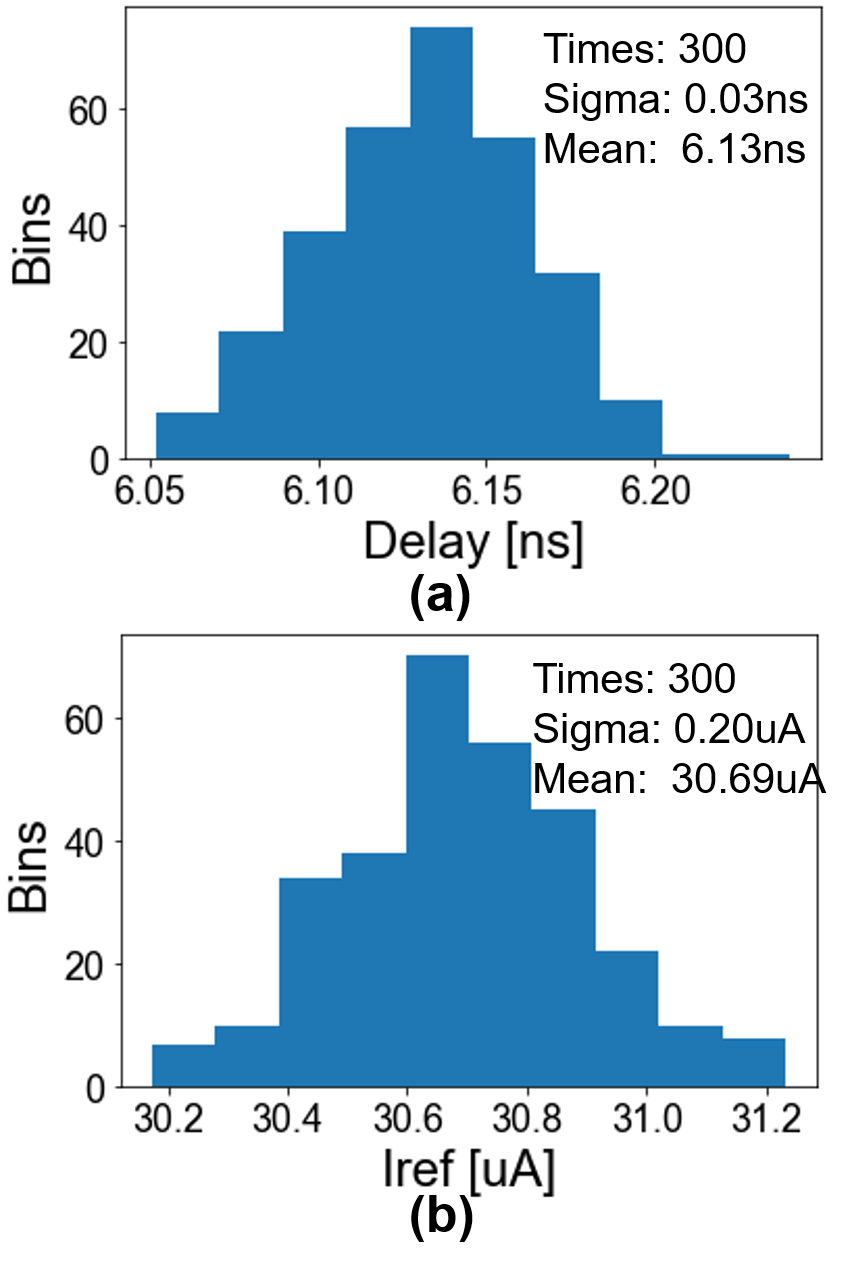
\includegraphics[width=0.35\textwidth]{figs/mc.png}
  \caption{(a) 
}
\label{monte}
\end{figure}

% GBWのシミュレーション結果
次に図\ref{iref_gbw}にて各種電流源を用いた時のPVTばらつきにおけるオペアンプのGBWシミュレーション結果を報告する。
BGR refはSS条件において電流減少してしまう効果があり理想電流源使用時と比べGBWは大きく減少しワーストコーナーではオペアンプGBWは30\%低下してしまう。このような状況だとオペアンプの設計マージンを拡大しなければならず、回路全体の消費電力が大きく増加してしまう。
一方でTBCSを用いるとPVT適応的な電流を生成する効果もあり、理想電流源とほぼオペアンプGBWは変わらない。ワーストコーナーでもGBW劣化は18\%とBGR refの半分程度に抑えることができ、オペアンプ設計マージンを抑えることができる。

%**・遅延器のミスマッチ効果(3σ)**
図\ref{monte}にある一定電流におけるCSI遅延とTBCSの生成電流の300回モンテカルロ解析結果を報告する。シミュレーションはTypical条件にてミスマッチを含むよう設定した。図\ref{monte}(a)にて示す10段遅延器のばらつきσは300psと小さく、生成電流結果に与える影響は少ない。そのため生成電流はほぼ抵抗素子のミスマッチによって決定される。抵抗素子は抵抗絶対値は大きくばらつくもののローカルミスマッチ特性は優れており、その影響も小さいことが図\ref{monte}(b)の結果から伺える。

\section{Conclusions}
To realize a fully adaptive noise scaling comparator, a VCO-based comparator with an eye-opening operation was introduced.  Even though the proposed VCO-based comparator was designed for a 13b ADC, this comparator can be used for further resolutions by carefully designing the jitter performance and the effective deadzone size. Moreover, since this comparator is mainly based on inverters and other simple logic cells, the comparator receives full benefits from process scaling. %Furthermore, the comparator characteristics can be analyzed with well-known knowledge of ring-oscillators. 

\bibliographystyle{IEEEbib}
\bibliography{main}


\begin{IEEEbiography}
[{
\includegraphics[width=1in,height=1.25in,clip,keepaspectratio]{bio/1.jpg}}]{Kentaro Yoshioka}
received his BS, MS, Ph.D degrees from Keio University, Japan. Currently, he is an Assistant Professor at Keio University. He worked with Toshiba during 2014-2021, developing circuitry for WiFi and LiDAR SoCs. During 2017-2018, he had been a visiting scholar at Stanford University, exploring efficient machine learning hardware and algorithms. 

Currently, Dr. Yoshioka serves as a technical program member of Symp. VLSI circuits conference. He was the recipient of ASP-DAC 2013 Special Feature Award, the A-SSCC 2012 Best Design Award, and 1st place winner of Kaggle 2020 Prostate Cancer Grade Assessment (PANDA) Challenge.
\end{IEEEbiography}

\end{document}
